
% 第1章 はじめに
\renewcommand{\baselinestretch}{1.5} % 行間の倍率指定
\section{はじめに}\label{sec:introduction}
\renewcommand{\baselinestretch}{1} % 行間の倍率指定

\par 近年インターネット普及により我々の身の周りでは数えきれないほど多くのウェブページが開発されている。NetCraftのWeb Server Surveyによると図\ref{fig-num_websites}に示すように2018年12月時点で世界中に15億を超えるウェブページが存在し、2008年の約10倍程度まで増加している\cite{webserver_survey}。さらにITRによると日本国内のウェブマーケティング市場は2016年度に売り上げ金額が16億円で前年比142.9\%増の急速な伸びとなり今後も引き続き市場拡大すると予想している\cite{itr_webmarket}。スマートフォンやタブレットなどのモバイル端末を一人一台所持するのが当たり前になった今日では、誰もがウェブページを日常で閲覧しており極めて重要性が高いと言える。

\begin{figure}[H]
    \centering
    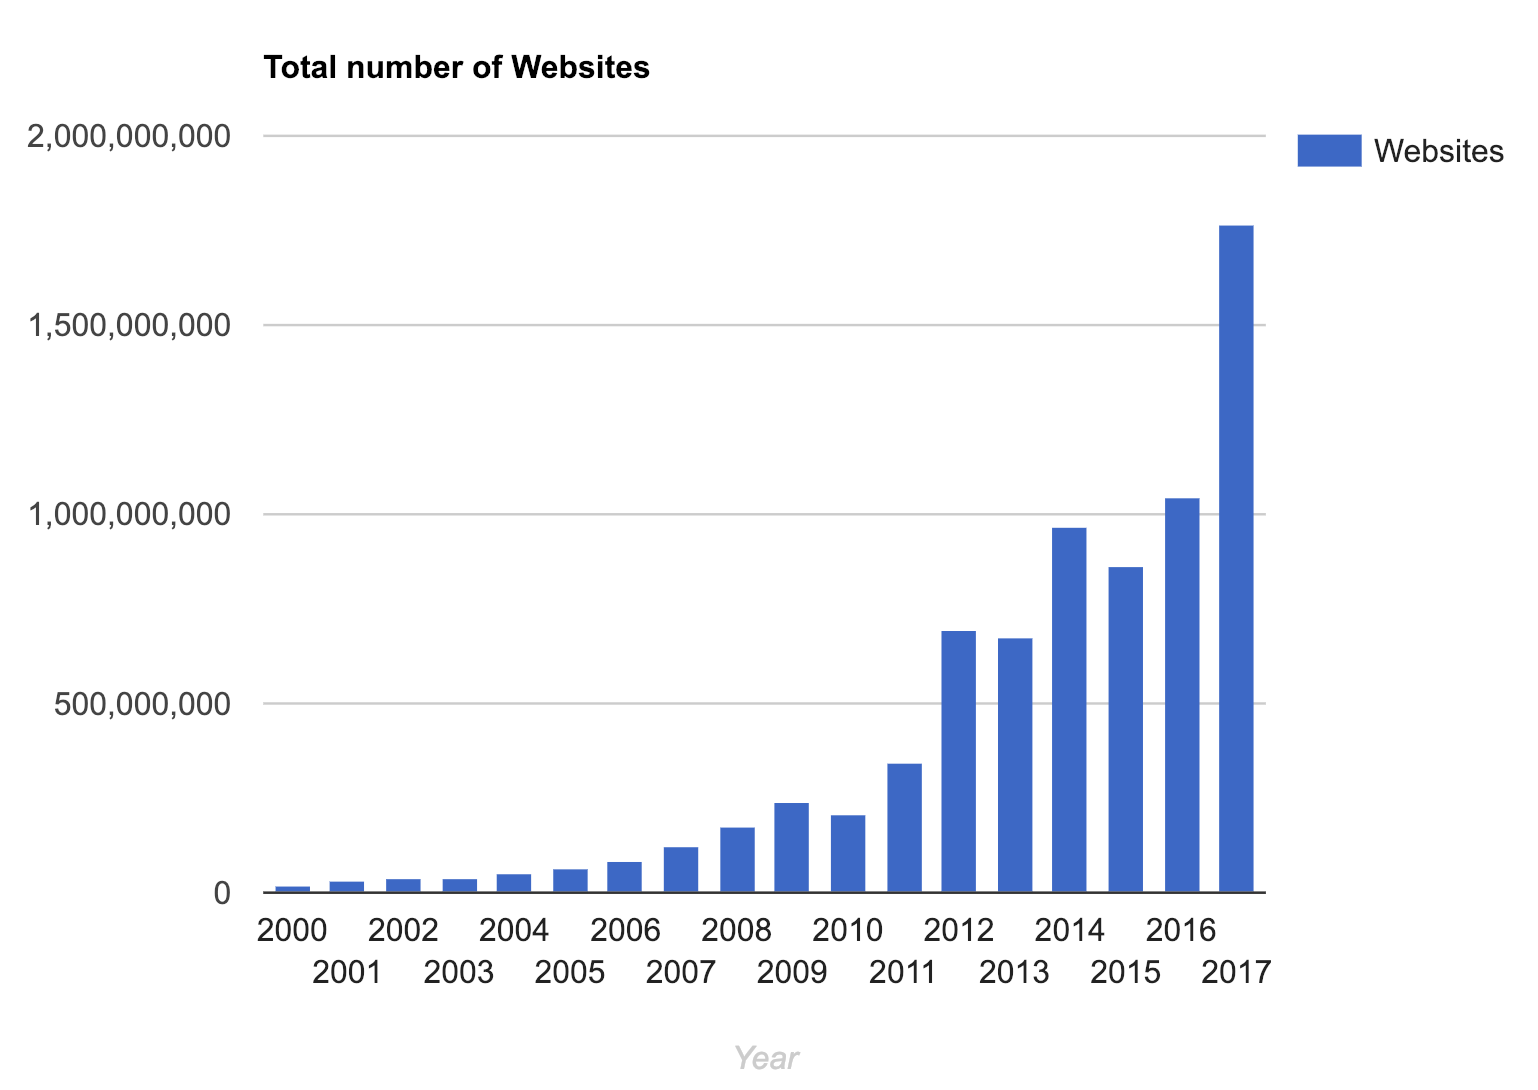
\includegraphics[width=8cm]{figures/01_number-of-websites.png}
    \caption{全世界のウェブページの数の推移\cite{internetlivestats}}
    \label{fig-num_websites}
\end{figure}

\par ウェブページを開発する時にデザイナーはユーザーに興味を持ってもらえるようなデザインかつ目的の要素や機能に簡単に到達できるようにレイアウトを設計する。しかしながら、実際にはデザインが良くても目的の要素を見つけづらいと感じたり使いづらいと感じるユーザビリティが低いウェブページは数多くある。ユーザーはユーザビリティが低いウェブページから離れやすい傾向があり、結果的にサービスの質や売り上げの低下に繋がってしまう。学生の論文共有サービスであるWriteWork\cite{writework}はヒートマップでウェブページの調査を行いCTAのテキストサイズの変更などのレイアウトの修正を行った結果有料サービスの売り上げが50\%も向上した\cite{writeworkabtest}。これはデザイナーの意思がしっかりとデザインに反映されず、デザイナーが見て欲しい情報とユーザーが実際に見ている情報にズレがあることが原因の一つである。

\par このような問題を未然に防ぐための一つの手法として、人の注視の引きつけやすさをヒートマップで示す顕著性マップをデザイナーに開発段階で示すことでユーザーが注目する可能性が高い領域を事前に知ることが効果的であると考える。風景や人の顔などの自然画像の顕著性マップ生成モデルに関する研究は多数存在するが、ウェブページに特化した顕著性マップの生成モデルについての研究はほとんど存在しない。また、顕著性マップを見ただけでは具体的にウェブページのどの要素が目立っているのか分かりづらい。

\par そこで本研究では、開発段階でウェブページ固有のレイアウトと顕著性マップを組み合わせることで要素単位で顕著度を計算することによるウェブページの重要領域の視覚化手法を提案する。ウェブページには画像やテキストなどの特有の要素が多数存在しており、正確な顕著性を予測するためにユーザーがウェブページを閲覧する際の視線データが必要となる。しかしながら、近年のモダンデザインに対応している視線データセットはウェブ上に公開されていないためオリジナルデータセットを作成する。作成したウェブページの視線データセットを用いて要素単位で顕著度を計算し、各要素の顕著度を可視化できる新たな顕著性マップとしてオリジナルの顕著領域マップを提案する。デザイナーがウェブページの開発・設計時にどの部分にユーザーの注目が集まるかを予想して、解析対象のウェブページ上に視覚的に描画することでウェブページの設計の効率化に繋がると考えている。

\par さらに、要素単位で顕著度のランキングを計算して特に顕著度が高い重要領域を1つの画像に集約したウェブページの集約図を提示する事によるページ内容理解支援手法を提案する。ユーザーが注目する可能性が高い顕著性が高い領域にはウェブページの重要な内容が含まれる事が多い為、該当領域を集約した図を提示する事でウェブページの内容の理解支援に繋がるのではないかと考えられる。

% 論文の構成
\par 本論文は、本章を含め全8章で構成される。第2章では本研究の背景となる視覚的顕著性と顕著性マップ生成モデルについて紹介し、第3章では本研究と関連する研究について述べる。第4章では本研究の特徴について述べ、第5章ではオリジナルで作成した視線データセットについて述べる。第6章では本研究の詳細について述べ、第7章で本研究の評価について述べる。最後に第8章おわりにで、全体の内容をまとめ今後の課題を述べる。